\chapter{Implementing policy-agnostic programming on the client side\label{chap:solution}}
We incorporated policy-agnostic programming into Javascript by adding constructs
defined for the Jeeves language as a subsystem. We chose Narcissus~\cite{narc},
a Javascript interpreter written in Javascript, to create the proof of concept.
Narcissus was built by its developers to be able to prototype new language features
for Javascript.

\section{Implementing faceted values in Narcissus}
Integral to implementing Jeeves is the implementation of faceted values. Our implementation
of faceted values derives heavily from the work done by Austin and Flanagan~\cite{Faceted}
and is inspired from the concept presented by Kerchove et al~\cite{Modular} for
``modular instrumentation'' of interpreters. They talk about how many dynamic analysis
approaches for information flow security have prototypes that are implemented in
very specific ways making it difficult to compare and reuse. They derive some
specific criteria to follow in order to achieve ``modular instrumentation'' using
the implementation~\cite{ZaphodFacets} of faceted values~\cite{Faceted} as a case
study. While we borrow a few ideas from this, our implementation does not follow
the criteria specified because achieving ``modular instrumentation'' would involve
non-trivial changes to the Narcissus interpreter making it out of scope of our problem.
What we did achieve is untangling of the concerns of the core interpreter for non-faceted
evaluation from the concerns of faceted evaluation. This makes it easier to relate
principles of faceted evaluation with the implemented prototype and also to extend
or reuse it.

Our implementation of faceted values is independent from the core Narcissus interpreter.
This involved making the core interpreter modular to be able to modify existing
evaluation mechanisms to behave differently for faceted values. The Narcissus interpreter
has an execute function which consists a switch case control flow that is set to
perform the appropriate set of operations based on the type of node identified by
the parser. Wherever there is need for faceted behavior, instead of making the core
interpreter code handle faceted behavior, we moved the part we would need to change
into a function and later override it to handle faceted behavior.
Figure~\ref{fig:facetif} shows how this overriding is implemented for the [F-IF-SPLIT]
evaluation rule. Here, \texttt{BaseExecContext} is an object that stores a copy of all the
fucntions from the core interpreter which we need to override. \texttt{ExecutionContext}
is an object from the core interpreter that keeps track of the current flow of execution.
\texttt{FacetExecContext} is the \texttt{ExecutionContext} object extended with
the \textit{pc} to help keep track of the influence of public or private facets
on the current flow of execution. In the \texttt{evalIfBlock} function, notice we
call the base \texttt{evalIfBlock} function if \texttt{cond} is not a faceted value.
Otherwise, we call the \texttt{evaluateEach} function which implements the [FA-SPLIT]
rules from Figure~\ref{fig:appRules}. We override behavior of the rest of the functions
in \texttt{BaseExecContext} in a similar manner.
\lstset{
  language=javascript,
  frame=single,
  breaklines=true,
  basicstyle=\footnotesize\ttfamily,
  numbers=left,
  extendedchars=true,
  tabsize=2
}
\begin{figure}
  \begin{lstlisting}
var BaseExecContext = {
  getValue : interpreter.ExecutionContext.prototype.getValue,
  putValue : interpreter.ExecutionContext.prototype.putValue,
  evalBinOp : interpreter.ExecutionContext.prototype.evalBinOp,
  evalUnaryOp : interpreter.ExecutionContext.prototype.evalUnaryOp,
  evalIfBlock : interpreter.ExecutionContext.prototype.evalIfBlock,
  evalDot : interpreter.ExecutionContext.prototype.evalDot,
  evalFunctionCall : interpreter.ExecutionContext.prototype.evalFunctionCall,
  runWhileLoop : interpreter.ExecutionContext.prototype.runWhileLoop
};

FacetExecContext.prototype.evalIfBlock = function(cond,thenPart,elsePart) {
  var execContext = FacetExecContext.current;
  if (cond instanceof FacetedValue) {
    evaluateEach(cond, function(v, x) {
      if (v) {
        interpreter.execute(thenPart, x);
      } else if (elsePart) {
        interpreter.execute(elsePart, x);
      }
    }, execContext);
  } else {
    BaseExecContext.evalIfBlock.call(this,cond,thenPart,elsePart);
  }
};
  \end{lstlisting}
  \caption{Independent implementation of faceted behavior for the ``if'' control flow}
  \label{fig:facetif}
\end{figure}

\begin{figure}
  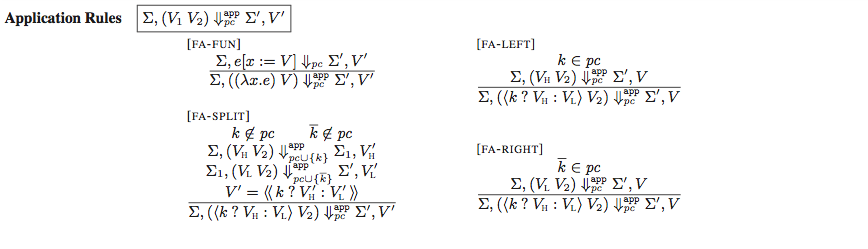
\includegraphics[scale=0.5, frame]{images/appRules}
  \caption{Function application rules~\cite{FacetedJeeves}}
  \label{fig:appRules}
\end{figure}

\section{Implementing Jeeves}
Once we had faceted values working, adding support for Jeeves constructs was pretty
straightforward. All of the Jeeves constructs are encapsulated in the prototype
of the \texttt{PolicyEnvironment} object which includes the [F-LABEL] and [F-RESTRICT]
evaluation rules as shown in Figure~\ref{fig:jeevesEval}. Every instance of the \texttt{PolicyEnvironment}
object has a \texttt{policyMap} that is used to store the `label':`policy' mapping.

\begin{figure}
  \centering
  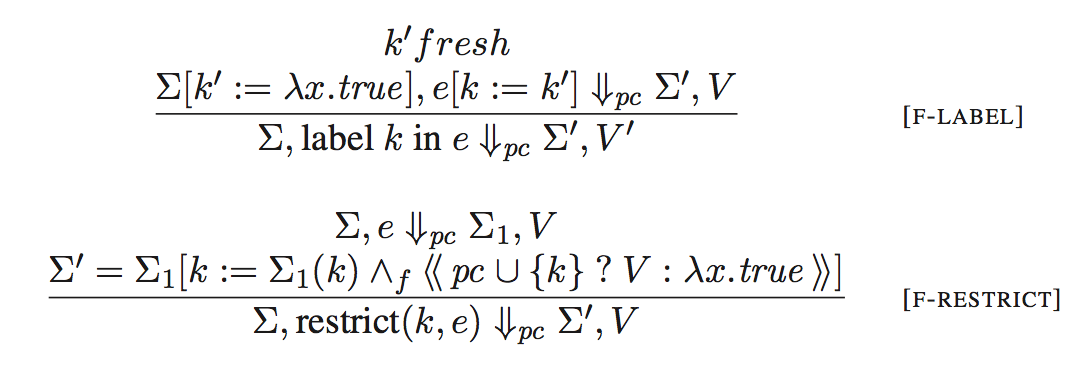
\includegraphics[scale=0.3, frame]{images/jeevesEval}
  \caption{Evaluation semantics for Jeeves labels and policies~\cite{FacetedJeeves}}
  \label{fig:jeevesEval}
\end{figure}

The Jeeves constructs available in the \texttt{PolicyEnvironment} prototype are:
\begin{enumerate}
  \item \texttt{mkLabel:} This function is roughly based on the [F-LABEL] rule. It
    creates a label and associates a default true policy to it.
  \item \texttt{restrict:} This function associates the given policy function to the
  given label in the \texttt{policyMap} of the current \texttt{PolicyEnvironment}.
  \item \texttt{mkSensitive:} This function creates a faceted value. It takes the
  label, private value, and public value as input and returns a faceted value. This
  function would only return the private value or the public value in cases where
  the current program counter contains the label or reverse of the label respectively.
  \item \texttt{concretize:} This function is used when the faceted value needs to
  be viewed in an output context. It takes the context object and faceted value
  as input and resolves the policies for all labels in the program counter of
  the faceted value recursively till it reaches a raw value with no facets.
  \item \texttt{partialConcretize:} Partial concretize is similar to the concretize
  function except it only resolves the policy associated with the first label of
  a possibly complex faceted value based on the given context object.
  Figure~\ref{fig:concretize} shows what the concretize and partialConcretize
  functions look like.
\end{enumerate}

\begin{figure}
  \begin{lstlisting}
function concretize(context, val) {
  if (val instanceof FacetedValue) {
    var label = head(val);
    var policy = this.policyMap[label];
    if (policy(context)) {
      return this.concretize(context, val.high);
    } else {
      return this.concretize(context, val.low);
    }
  } else {
    return val;
  }
}
function partialConcretize(context, val) {
  if (val instanceof FacetedValue) {
    var label = head(val);
    var policy = this.policyMap[label];
    if (policy(context)) {
      val = val.high;
    } else {
      val = val.low;
    }
  }
  return val;
}
  \end{lstlisting}
  \caption{Concretize and partialConcretize function definitions}
  \label{fig:concretize}
\end{figure}

\subsection{Using Jeeves constructs}
Figure~\ref{fig:JeevesExamples} shows two test cases of how the Jeeves constructs
listed above would be used. Note, \texttt{policyEnv} is an instance of the
\texttt{PolicyEnvironment} prototype.

In \texttt{testPolicyComplexFacets}, we are constructing complex faceted values
with two principals/labels and have two different policies for each respectively.
The call to \texttt{concretize} at the end shows what a context object would look
like in this case. The faceted value stored in \texttt{a} in notation looks like
this: $\langle x~?~\langle y~?10~:~15 \rangle~:~0 \rangle$.

In \texttt{testPartialConcretize}, we are using \texttt{partialConcretize} with
two different context objects. This type of usage would be ideal for a client-server
interaction where you can have different context objects for the server and client-side
respectively. Note, in the example the policies associated with the two labels are
expecting different properties in the context object passed to them.

\begin{figure}
  \begin{lstlisting}
 function() testPolicyComplexFacets{
  var x = policyEnv.mkLabel("x");
  policyEnv.restrict(x, function (context) {
    return context.val1 === 22 && context.val2 === 21;
  });

  var y = policyEnv.mkLabel("y");
  policyEnv.restrict(y, function (context) {
    return context.val2 === 22;
  });
  var a = policyEnv.mkSensitive(x, policyEnv.mkSensitive(y, 10, 15), 0);
  return assertEquals(policyEnv.concretize({val1: 22, val2: 21}, a), 15);
};

function testPartialConcretize() {
  var x = policyEnv.mkLabel("x");
  policyEnv.restrict(x, function (context) {
    return context.val1 === 22 && context.val2 === 21;
  });

  var y = policyEnv.mkLabel("y");
  policyEnv.restrict(y, function (context) {
    return context.otherVal = 44;
  });
  var a = policyEnv.mkSensitive(x, policyEnv.mkSensitive(y, 10, 15), 0);

  var result1 = assertEquals(policyEnv.partialConcretize({val1: 22, val2: 21}, b).toString(), "{y?10:15}");
  var result2 = assertEquals(policyEnv.partialConcretize({val:22}, b), 0);
  return result2 && result1;
};
  \end{lstlisting}
  \caption{Example usage of Jeeves constructs}
  \label{fig:JeevesExamples}
\end{figure}

\section{Policy agnostic programming in dom.js}
Web browsers have an implementation of the DOM to allow scripts to
access and manipulate content. We add faceted values and policy agnostic-programming
constructs to the DOM implementation to show how it can be used to prevent
sensitive data from leaking.

We use dom.js~\cite{dom.js} which is a DOM implementation written in
Javascript. This makes it possible for us to parse it using Narcissus
and make DOM components available to scripts just like a web browser would. The
advantages of using dom.js is highlighted by Austin et al~\cite[Section 9.3]{TOPLAS}
since it makes it possible to include faceted values in the DOM and track flow of
private information on the web browser.

We first identify entry and exit points in the DOM that have potential
to leak sensitive data such as when the \texttt{setAttribute} and \texttt{getAttribute}
functions of an element are called; when a \texttt{Text} node is created
and appended to a DOM and when the \texttt{innerHTML} property of an element
is used to access the text within an element; and finally when an
\texttt{XMLHttpRequest} is made to load an external script, image, or other media.

Note here, the \texttt{setAttribute} function and creation of the \texttt{textNode}
are entry points into the DOM. Here, we have to be careful not to render sensitive
information onto unwanted components like the \textit{src} attribute of an image
or script tag. We discuss such a scenario in Section~\ref{sec:exfil}. On the
other hand, once a value is rendered onto the DOM, a script may try to access rendered
values using the \texttt{getAttribute} function and the \texttt{innerHTML} property.

We introduce an instance of the \texttt{PolicyEnvironment} prototype to the window
object. This would give access to Jeeves constructs within the DOM along with a
\texttt{policyMap} for each web page. We also introduce a \texttt{facetedValueMap}
available as a global store that associates textNodes or attributes of elements
with corresponding faceted values. The \texttt{facetedValueMap} is of
type WeakMap that provides a loose mapping from objects to values~\cite{WeakMap}.

Figure~\ref{fig:createTextNode} shows how creation of a text node for faceted values
is handled within the DOM. The function \texttt{createTextNode} would create a
node that would eventually be rendered onto a web page. At this point, we need to
decide which facet of a faceted value should be rendered. Note, in the function
we are calling \texttt{isFaceted} which we have made available in the global scope.
If the input to \texttt{createTextNode()} is faceted then we concretize that value
to get a raw value to be rendered. Additionally, we add the faceted value itself
to the \texttt{facetedValueMap} with the textNode as key. We have added similar
code in the \texttt{setAttribute} function of an element with one distinction to
the object that is used as key for the \texttt{facetedValueMap}. Here we cannot
use the node as the key since we need to have different keys for different
attributes of an element. So we created an object using the id of the element and
the attribute name as follows:
\indent\texttt{facetedValueMap[\{id:this.id, attr:attributeName\}] = value;}
\noindent

Figure~\ref{fig:innerHTML} shows how access to the \texttt{innerHTML} property of
an element would return a faceted value instead of the actual content that was
rendered on the web page (lines 7-9). Note, \texttt{serialize} is a function
called by the \texttt{innerHTML} getter. We have similar code to return a faceted
value in the \texttt{getAttribute} function of an element with the key as shown
above for the \texttt{setAttribute} function.

\begin{figure}
  \begin{lstlisting}
// Convert the children of a node to an HTML string.
// This is used by the innerHTML getter
serialize: constant(function() {
  var s = "";
  for(var i = 0, n = this.childNodes.length; i < n; i++) {
    var kid = this.childNodes[i];
    if (kid in facetedValueMap) {
      return facetedValueMap[kid];
    }
    .
    .
    .
  }
  .
  .
  .
}
  \end{lstlisting}
  \caption{Return faceted value if exists when the innerHTML property is accessed}
  \label{fig:innerHTML}
\end{figure}

\begin{figure}
  \begin{lstlisting}
createTextNode: function createTextNode(data) {
  var dataString = data;
  var dataIsFaceted = isFaceted(data);
  if (dataIsFaceted) {
    dataString = window.policyEnv.concretize(null, data);
  }
  var textNode = unwrap(this).createTextNode(String(dataString));
  if (dataIsFaceted) facetedValueMap[textNode] = data;
  return wrap(textNode);
},
  \end{lstlisting}
  \caption{Persisting faceted values for createTextNode}
  \label{fig:createTextNode}
\end{figure}


\section{A data exfiltration case study \label{sec:exfil}}
We present a simple data exfiltration attack that succeeds in exfiltrating sensitive
data from the a web page to a server that the attacker owns. A direct XMLHttpRequest
to do this would be prevented by the same-origin policy of the web browser but there
is a simple workaround. The same-origin policy does not restrict the source of a
script or image tag. Although you may use CSP to restrict sources, it becomes difficult
to track what images sources to allow and so web developers tend to keep the CSP
of \textit{img-src} as a wildcard (*) allowing all urls for images.

The Figure~\ref{fig:salaryMgr} shows a screenshot of a simple web page we created
that shows the salary of the user currently logged-in and salaries of his subordinates.
The helpful greeting at the top right corner along with the nice background color
is a due to a third-party library that Trudy suggested would be a nice addition
to make the otherwise mundane user interface better. Turns out the third-party
library also does some malicious activity along with these ``colorful'' additions.
Figure~\ref{fig:trudyLib} shows the code of the third party library. Here, lines
14-15 would get the message that displays Manny's salary. Lines 17-20 extract manny's
name and salary and line 21 would result in an attempt to asynchronously load an
image with the name ``Manny\_10000.jpg'' from ``localhost:8081'' which is not the
same as the origin of the web page as shown in the address bar in Figure~\ref{fig:salaryMgr}.
This would happen anytime Manny clicks anywhere on the web page. Now, although there
is no image with the name ``Manny\_10000.jpg'' at ``localhost:8081'', the attacker
can access Manny's salary by checking their http access logs as shown in
Figure~\ref{fig:accessLog}.

\begin{figure}
  \centering
  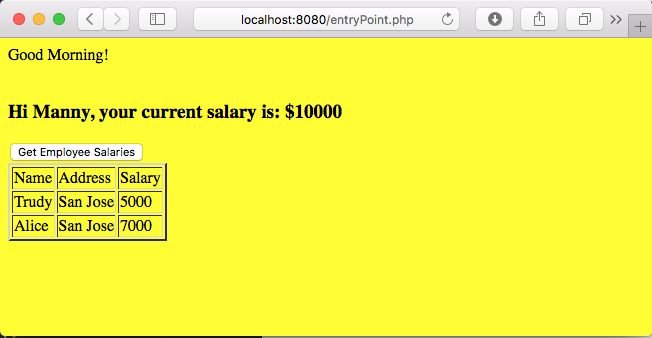
\includegraphics[scale=0.5, frame]{images/scrShot1}
  \caption{Web page that displays employee salaries}
  \label{fig:salaryMgr}
\end{figure}

\begin{figure}
  \begin{lstlisting}
var d = new Date();
var time = d.getHours();
var greetingNode = document.getElementById("greeting");
var message = "Good day!";
document.body.style.fontStyle.color = "black";
//This section sets background color and greeting based on the time
.
.
.
var welcomeText = document.createTextNode(message);
greetingNode.appendChild(welcomeText);
//Malicious code:
document.addEventListener("click", function () {
  var salaryField = document.getElementById("OwnSalary");
  var text = salaryField.innerHTML;
  var malImg = document.createElement("img");
  var commaPos = text.indexOf(",");
  var dollarPos = text.indexOf("$");
  var name = text.slice(3,commaPos);
  var salary = text.slice(dollarPos+1);
  malImg.setAttribute("src","http://localhost:8081/" + name + "_" + salary + ".jpg");
  //The following would violate the same origin policy:
  //$.post('http://localhost:8081/exfil.php',{message:text});
});
  \end{lstlisting}
  \caption{Third Party library with exfiltration code}
  \label{fig:trudyLib}
\end{figure}

\begin{figure}
  \centering
  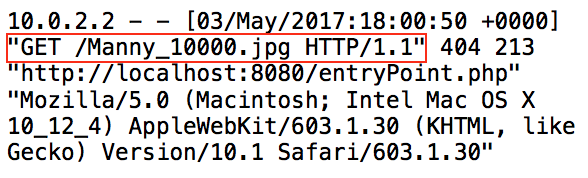
\includegraphics[scale=0.5, frame]{images/accessLog}
  \caption{Access log entry giving Manny's salary information to the attacker}
  \label{fig:accessLog}
\end{figure}

Now let's look at how policy-agnostic programming controls in the DOM would prevent
such an attack. Figure~\ref{fig:displaySalary} shows a code snippet of the code
that would display a message similar to the one shown in Figure~\ref{fig:salaryMgr}.
Note, the string concatenation in the code would produce a faceted value of the
form:\\
\indent \texttt{<"n"?}
  \texttt{<"s"?"Manny's Salary is:10000":"Manny's Salary is:0">:}\\
  \indent\indent\texttt{<"s"?"JonDoe's Salary is:10000":"Manny's Salary is:0">~>}
\noindent \eject
So, with the correct policies in place, the message displayed on the web page would
be ``Manny's Salary is:10000'' and the image request would be for ``JonDoe\_0.jpg''.

\begin{figure}
  \begin{lstlisting}
//fName is a faceted value of the form <"n"?"Manny":"JonDoe">
//fSalary is a faceted value of the form <"s"?"10000":"0">
document.body.appendChild(document.createTextNode(fName + "'s Salary is:" + fSalary));
  \end{lstlisting}
  \caption{Code that would set the display message on the web page}
  \label{fig:displaySalary}
\end{figure}

A sample policy function to protect salary data is shown in Figure~\ref{fig:policyEx}.
Here we have three conditions that would determine if the salary of a user is safe
to be revealed to the output context. We can certainly have more powerful policies
which can be tailored to the target application.

\begin{figure}[H]
  \begin{lstlisting}
function (ctxt) {
  if (ctxt.urlDomain && ctxt.urlDomain != "myCorp.org") {
    return false;
  } else if (ctxt.User && ctxt.User.role != "admin") {
    return false;
  } else if (ctxt.time && ctxt.time.hour > 17) {
    return false;
  }
  return true;
}
  \end{lstlisting}
  \caption{Example of a policy function for protecting salary data from being exfiltrated}
  \label{fig:policyEx}
\end{figure}
